\chapter{Cartomancia con Naipes Ingleses}\label{english-playing-card-cartomancy}

\begin{center}
  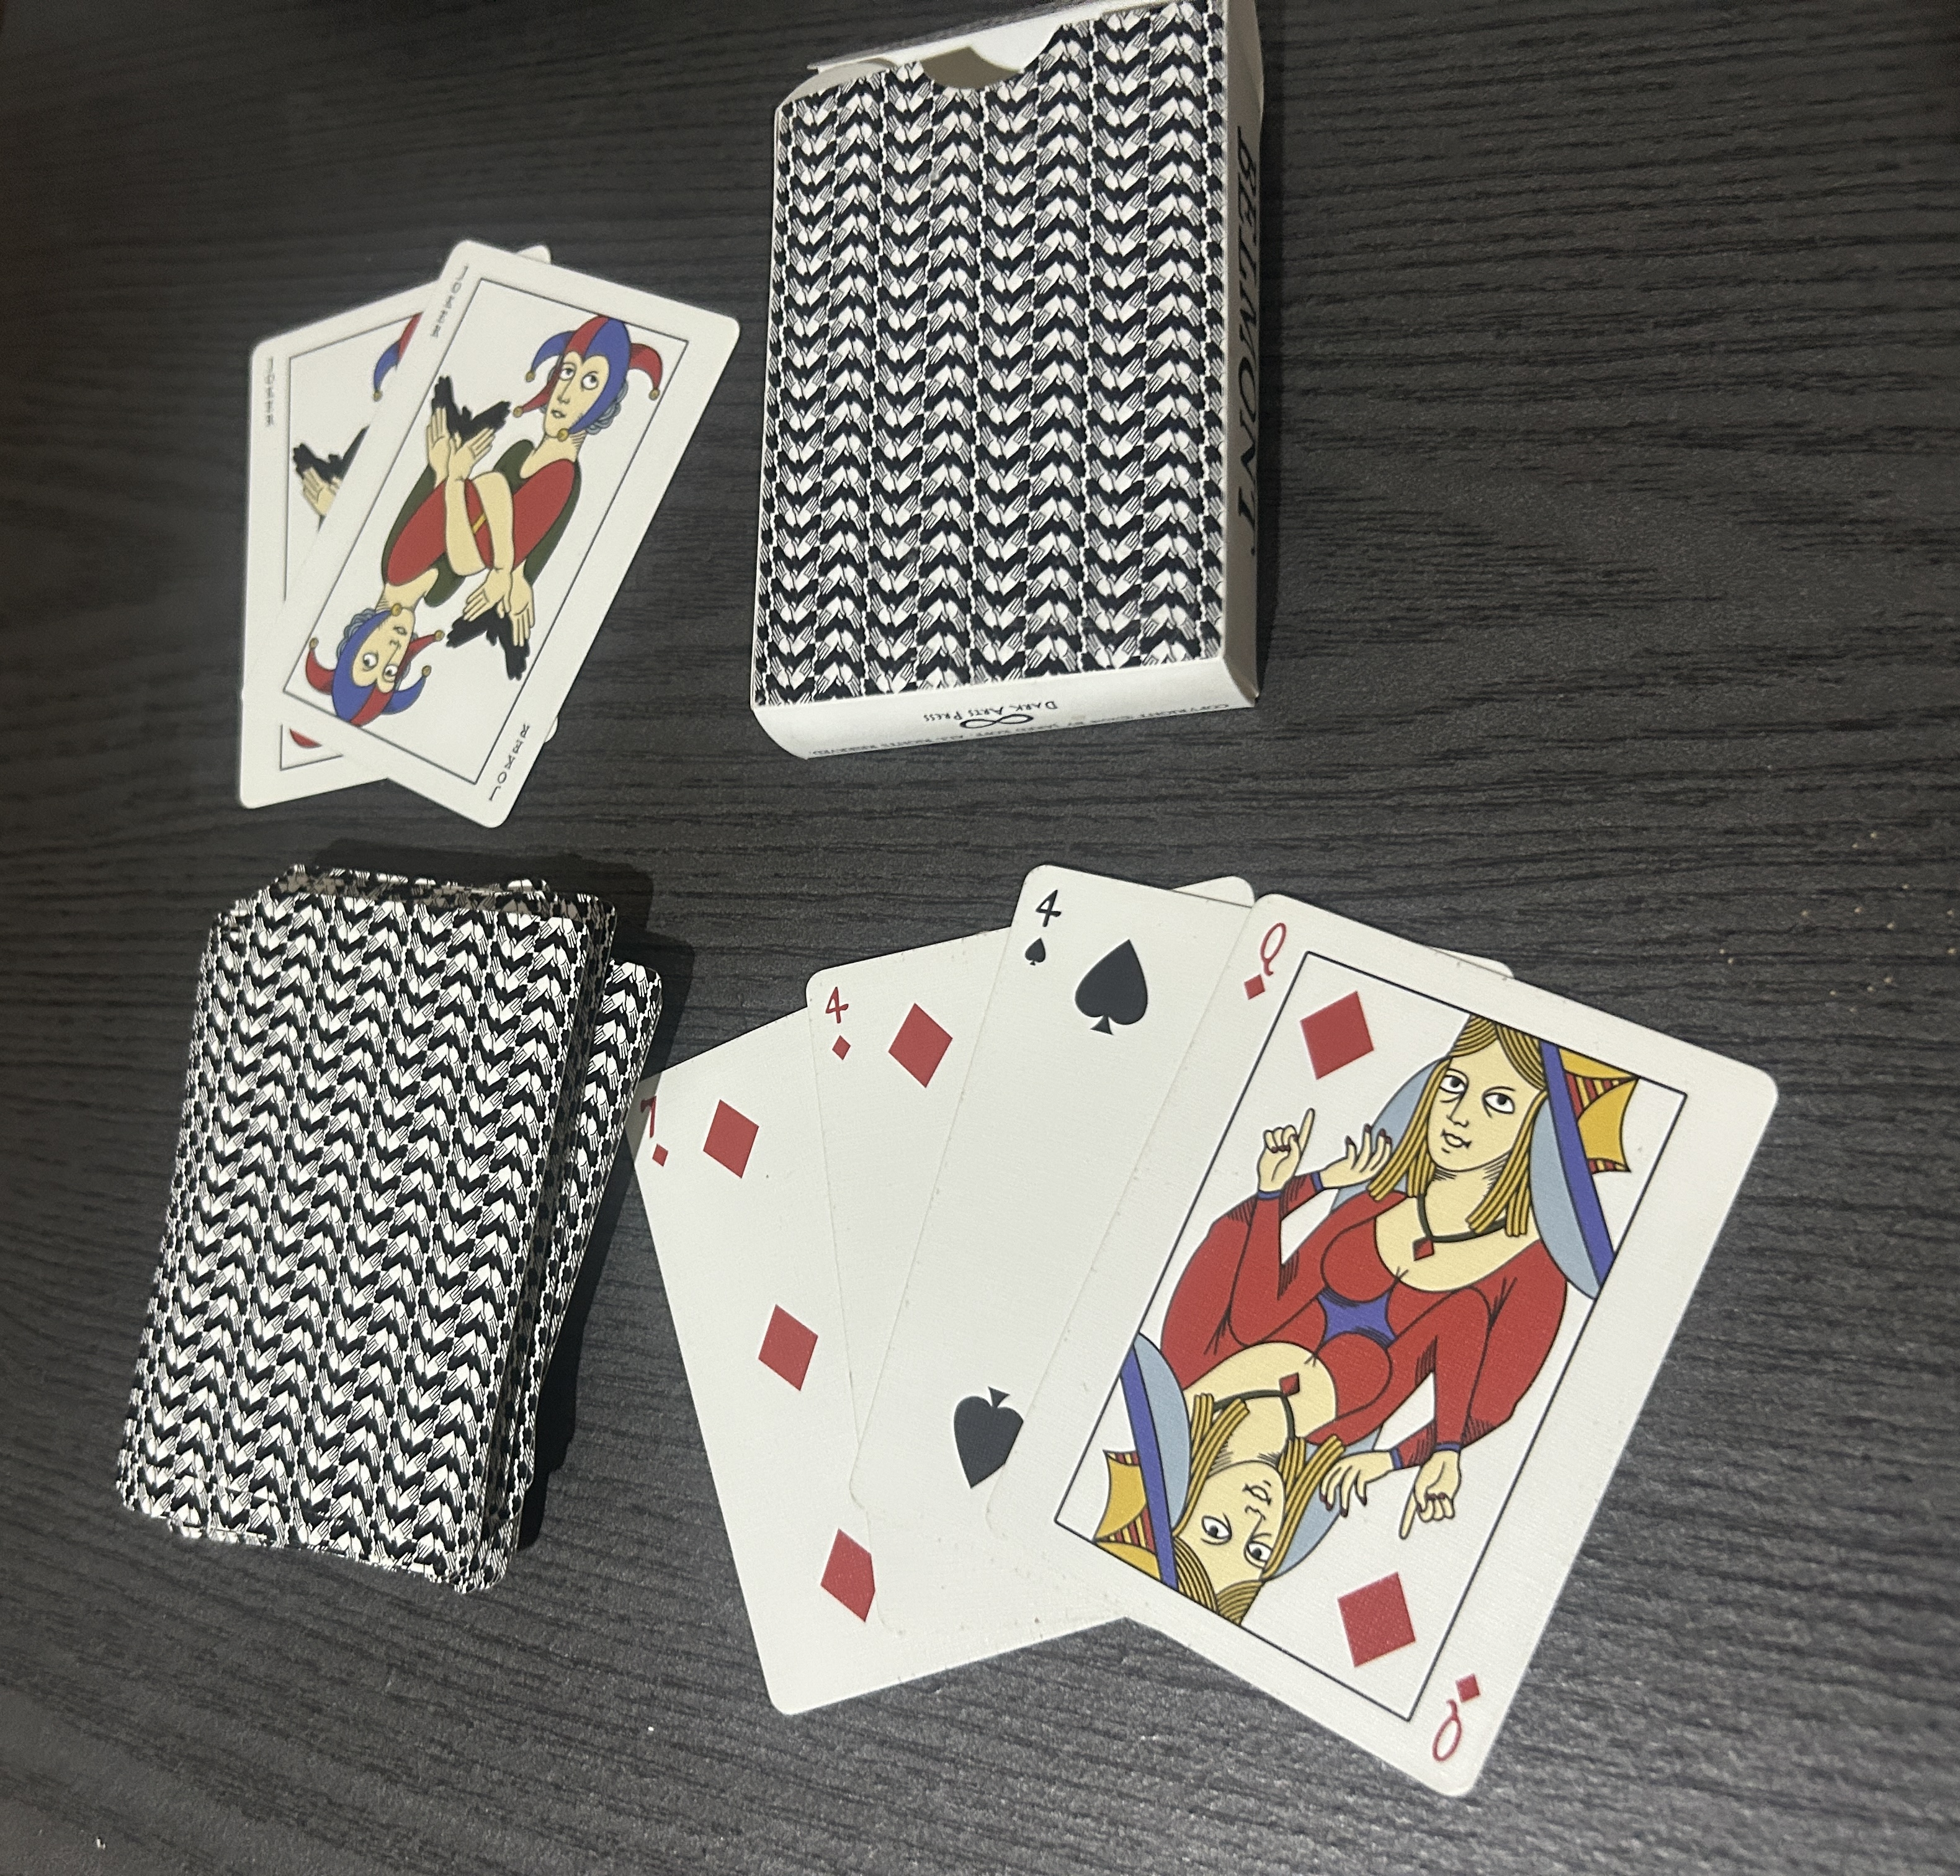
\includegraphics[width=0.85\textwidth,keepaspectratio]{img_playing_cards.jpg}
\end{center}

\section{Principios de Funcionamiento}\label{operating-principles}

Este sistema opera a nivel de las circunstancias, las relaciones y el movimiento temporal: la textura de la vida cotidiana. Responde a preguntas sobre qué está pasando realmente y a quién.

El As es la carta más alta, no la primera. Es la expresión más plena del poder del palo, no su semilla.

Se incluye un comodín. Ver más abajo.

\begin{center}\rule{0.5\linewidth}{0.5pt}\end{center}

\section{Los Palos}\label{the-suits}

\textbf{Corazones} --- el ámbito personal y emocional. El amor, la amistad, el hogar, la familia, la felicidad, lo que más apreciamos. El palo de la vida interior y las relaciones íntimas. Favorable en casi cualquier posición. Cuando los Corazones dominan una tirada, la pregunta se centra básicamente en cómo se sienten las personas y qué es lo que desean emocionalmente.

\textbf{Diamantes} --- el ámbito material y comunicativo. El dinero, los bienes, los asuntos prácticos, los mensajes, las noticias, la correspondencia, los viajes por motivos prácticos. También: regalos, ofertas, transacciones. Los Diamantes describen el movimiento de las cosas y la información en el mundo. De carácter neutro ---ni afortunados ni desafortunados por naturaleza---, describen la realidad material tal y como es.

\textbf{Tréboles} --- la esfera de la iniciativa y el esfuerzo. Trabajo, ambición, negocios, actividad social, construcción, crecimiento a través de la acción. Generalmente favorables ---una tirada con muchos Tréboles indica movimiento, iniciativa, cosas que se están construyendo o logrando. El palo de lo que hacés que suceda gracias a tu propio esfuerzo.

\textbf{Picas} --- la esfera del desafío y las consecuencias. Conflicto, oposición, retrasos, dificultades, pérdidas, finales, verdades duras pero necesarias. No son simplemente negativas: las Picas describen lo que tiene un coste, lo que hay que afrontar, lo que no se puede evitar. Son el palo de las cosas serias. Una tirada sin Picas es a veces una tirada que no cuenta toda la verdad.

\begin{center}\rule{0.5\linewidth}{0.5pt}\end{center}

\section{Equilibrio entre Palos}\label{suit-balance}

Antes de leer las cartas individuales, fijate en la distribución por palos:

\begin{itemize}
\tightlist
\item
  Predominio de Corazones: una situación emocional en su esencia
\item
  Predominio de Diamantes: una situación material o comunicativa
\item
  Predominio de Tréboles: algo que se está construyendo o por lo que se está trabajando
\item
  Predominio de Picas: una situación seria con costes reales
\end{itemize}

Vale la pena notar la ausencia de Picas en una tirada: o bien la situación realmente no tiene ninguna dimensión difícil, o bien el consultante no está haciendo la pregunta correcta.

\begin{center}\rule{0.5\linewidth}{0.5pt}\end{center}

\section{Lógica Numerológica}\label{numerological-logic}

Los números tienen un carácter cualitativo inherente que se aplica de forma coherente en los cuatro palos. No se trata de numerología cabalística ---no se deriva de los Sephiroth. Es algo empírico y asociativo, acumulado a lo largo de siglos de uso práctico. El palo te indica el ámbito; el número te dice lo que está sucediendo dentro de ese ámbito.

Entender el carácter del número te permite deducir el significado de forma intuitiva cuando una carta concreta resulta incierta, y te ayuda a leer la lógica de una secuencia cuando aparecen varias cartas del mismo número en una tirada.

\textbf{As} --- fuerza máxima. El poder del palo en su máxima expresión. Único, indivisible, definitivo. Un punto álgido, no un comienzo. Lo que sea que gobierne el palo, el As dice: esto importa completamente.

\textbf{Dos} --- dualidad. Un encuentro, una unión, una elección entre dos caminos. Dos fuerzas en relación. El número del encuentro: algo está encontrándose con algo más.

\textbf{Tres} --- multiplicación, fuerza social, la entrada de un tercer elemento. Dos se convierte en tres. El número de los grupos, de los primeros resultados que aparecen.

\textbf{Cuatro} --- consolidación. Lo que se puso en marcha ha encontrado una forma estable. Puede ser tranquilizador o estancado según el palo y el contexto.

\textbf{Cinco} --- perturbación. El cuatro estable se ha visto alterado. El cambio es inevitable. El número de la inestabilidad.

\textbf{Seis} --- resolución gradual. Tras la perturbación del cinco, las cosas empiezan a avanzar hacia el equilibrio. No es la llegada, sino el movimiento hacia ella.

\textbf{Siete} --- el obstáculo, la prueba, lo que requiere un manejo cuidadoso. No es una catástrofe, sino la fricción que ralentiza o complica. A menudo una advertencia: algo necesita atención antes de que empeore.

\textbf{Ocho} --- movimiento y llegada. Las cosas se aceleran, llegan noticias, se acercan personas o acontecimientos. El número de lo que está en movimiento hacia el consultante o hacia la resolución.

\textbf{Nueve} --- casi completado, intensidad. El carácter del palo actuando con una fuerza casi máxima. Un paso antes del final o la crisis.

\textbf{Diez} --- finalización y resultado. El ciclo ha seguido su curso. Lo que fuera hacia lo que se dirigía el palo ha llegado.

\textbf{Sobre varias cartas del mismo número en una tirada:} cuando dos o más cartas comparten un número, esa cualidad es enfática en la lectura. Dos cuatros: estancamiento profundo o estabilidad profunda. Tres sietes: obstáculos significativos que requieren atención seria. Cuatro nueves: una situación en punto de crisis en múltiples ámbitos simultáneamente. Lee primero el carácter del número, luego los palos para saber qué ámbitos se ven afectados.

\begin{center}\rule{0.5\linewidth}{0.5pt}\end{center}

\section{Las Cartas Numéricas}\label{the-number-cards}

\subsection{Ases --- la expresión más plena del poder del palo}\label{aces--the-fullest-expression-of-the-suits-power}

\begin{itemize}
\tightlist
\item
  \textbf{As de Corazones}: el hogar, el amor profundo, una verdad emocional central
\item
  \textbf{As de Diamantes}: un acontecimiento financiero importante, un mensaje o carta importante
\item
  \textbf{As de Tréboles}: gran éxito, una nueva empresa significativa
\item
  \textbf{As de Picas}: la carta más seria de la baraja. Un gran desafío, un final significativo, la verdad más dura de la lectura. No significa muerte física sino el tipo de final que lo cambia todo.
\end{itemize}

\subsection{Doses --- asociación, dualidad, elección, encuentro, acuerdo}\label{twos--partnership-duality-choice-meeting-agreement}

\begin{itemize}
\tightlist
\item
  \textbf{2 de Corazones}: afecto mutuo, una asociación exitosa en el amor
\item
  \textbf{2 de Diamantes}: una asociación o acuerdo financiero, a veces una partida
\item
  \textbf{2 de Tréboles}: oposición o rumores que frustran una empresa, una asociación difícil en el trabajo
\item
  \textbf{2 de Picas}: división, separación, una separación de caminos ---física o emocional
\end{itemize}

\subsection{Treses --- un tercero, grupos, situaciones sociales, resolución o complicación inicial}\label{threes--a-third-party-groups-social-situations-initial-resolution-or-complication}

\begin{itemize}
\tightlist
\item
  \textbf{3 de Corazones}: celebración, buena compañía, una reunión feliz, felicitaciones
\item
  \textbf{3 de Diamantes}: asuntos legales, disputas domésticas, a veces un tercero en una situación financiera
\item
  \textbf{3 de Tréboles}: un segundo matrimonio o complicación romántica, éxito social
\item
  \textbf{3 de Picas}: separación, partida, lágrimas ---tristeza con dimensión social
\end{itemize}

\subsection{Cuatros --- estabilidad, consolidación, descanso; también estancamiento}\label{fours--stability-consolidation-rest-also-stagnation}

\begin{itemize}
\tightlist
\item
  \textbf{4 de Corazones}: un viaje, viaje por razones personales, un cambio en las circunstancias domésticas
\item
  \textbf{4 de Diamantes}: herencia, un cambio financiero inesperado, dinero de una fuente inesperada
\item
  \textbf{4 de Tréboles}: un cambio de planes, una advertencia contra la incaución, inestabilidad en la empresa
\item
  \textbf{4 de Picas}: enfermedad, convalecencia, un período de descanso o retirada forzada
\end{itemize}

\subsection{Cincos --- inestabilidad, cambio, perturbación de lo establecido}\label{fives--instability-change-disruption-of-what-was-established}

\begin{itemize}
\tightlist
\item
  \textbf{5 de Corazones}: celos, incertidumbre en el amor, un corazón voluble, indecisión
\item
  \textbf{5 de Diamantes}: buenas noticias sobre el dinero, un mensaje próspero
\item
  \textbf{5 de Tréboles}: nuevas amistades, nuevas alianzas, ayuda que llega de un lugar inesperado
\item
  \textbf{5 de Picas}: pérdida, duelo, dolor, algo que se nos arrebata
\end{itemize}

\subsection{Seises --- movimiento gradual, cosas que se estabilizan o resuelven lentamente}\label{sixes--gradual-movement-things-stabilizing-or-resolving-slowly}

\begin{itemize}
\tightlist
\item
  \textbf{6 de Corazones}: buena fortuna inesperada, un regalo del pasado, algo que regresa
\item
  \textbf{6 de Diamantes}: un matrimonio o unión temprana, mejora de los asuntos financieros, una reconciliación
\item
  \textbf{6 de Tréboles}: éxito empresarial, un viaje comercial que da frutos
\item
  \textbf{6 de Picas}: un viaje por agua, viaje, una transición de un estado a otro ---a menudo mejora tras dificultades
\end{itemize}

\subsection{Sietes --- obstáculos, pruebas, cosas que requieren paciencia o acción cuidadosa}\label{sevens--obstacles-tests-things-requiring-patience-or-careful-action}

\begin{itemize}
\tightlist
\item
  \textbf{7 de Corazones}: alguien poco fiable, una promesa que puede no mantenerse, agradable pero inconstante
\item
  \textbf{7 de Diamantes}: un niño, una pequeña discusión sobre el dinero, algo pequeño que interrumpe los asuntos materiales
\item
  \textbf{7 de Tréboles}: imprudencia, temeridad, prosperidad amenazada por acciones descuidadas
\item
  \textbf{7 de Picas}: pérdida por robo, traición, una advertencia sobre la confianza
\end{itemize}

\subsection{Ochos --- movimiento, noticias que llegan, cosas que se aceleran o cristalizan}\label{eights--movement-news-arriving-things-accelerating-or-crystallizing}

\begin{itemize}
\tightlist
\item
  \textbf{8 de Corazones}: un viaje por amor o placer, una visita, viajar hacia alguien
\item
  \textbf{8 de Diamantes}: un viaje corto, un pequeño viaje práctico, una diligencia de negocios
\item
  \textbf{8 de Tréboles}: la aproximación de una persona de pelo oscuro, viaje, movimiento en asuntos de trabajo
\item
  \textbf{8 de Picas}: decepción, tristeza, oposición de alguien con autoridad, planes bloqueados
\end{itemize}

\subsection{Nueves --- casi completados, resultados fuertes, el carácter del palo con intensidad casi máxima}\label{nines--near-completion-strong-outcomes-the-suit-character-at-near-maximum-intensity}

\begin{itemize}
\tightlist
\item
  \textbf{9 de Corazones}: la carta del deseo. La carta más afortunada de la baraja. Lo que el consultante más desea.
\item
  \textbf{9 de Diamantes}: una sorpresa, noticias inesperadas ---la dirección la determinan las cartas que la rodean
\item
  \textbf{9 de Tréboles}: fortuna inesperada, un logro significativo, la recompensa de la perseverancia
\item
  \textbf{9 de Picas}: enfermedad, mala suerte, la carta más oscura después del As de Picas. Dificultad profunda.
\end{itemize}

\subsection{Dieces --- finalización, resultados plenos, el final de un ciclo}\label{tens--completion-full-outcomes-the-end-of-a-cycle}

\begin{itemize}
\tightlist
\item
  \textbf{10 de Corazones}: buena fortuna, felicidad, el mejor resultado posible para asuntos personales y emocionales
\item
  \textbf{10 de Diamantes}: un viaje, un cambio de residencia, un cambio financiero significativo
\item
  \textbf{10 de Tréboles}: buena fortuna inesperada a través de la empresa, una ganancia inesperada a través del trabajo
\item
  \textbf{10 de Picas}: pena, desgracia, lágrimas. También: finalización de un ciclo difícil, el final de un camino duro.
\end{itemize}

\begin{center}\rule{0.5\linewidth}{0.5pt}\end{center}

\section{Las Cartas de la Corte}\label{the-court-cards}

Las cartas de la corte representan a personas en la vida del consultante, o aspectos del consultante, según el contexto. El sistema de colores es una ayuda mnemotécnica para el tipo de carácter, no una descripción física literal: usá el carácter del palo como identificador principal.

\textbf{Cartas de la corte de Corazones} --- tez clara, pelo claro, ojos claros. Afectuosos, emocionales, artísticos. \textbf{Cartas de la corte de Diamantes} --- tez clara a media, pelo claro a medio. Prácticos, materialistas, activos. \textbf{Cartas de la corte de Tréboles} --- tez morena, pelo oscuro, ojos oscuros. Ambiciosos, enérgicos, apasionados. \textbf{Cartas de la corte de Picas} --- serios, autoritarios, asociados con asuntos difíciles y poder.

\subsection{Reyes --- hombres maduros, figuras de autoridad, hombres de experiencia o poder}\label{kings--mature-men-authority-figures-men-of-expertise-or-power}

\begin{itemize}
\tightlist
\item
  \textbf{Rey de Corazones}: un hombre amable, gentil y generoso. Afectuoso, de buen carácter. Un amigo o compañero fiable.
\item
  \textbf{Rey de Diamantes}: un hombre obstinado y poderoso. Con éxito en los negocios, no siempre fiable. Observá sus acciones más que sus palabras.
\item
  \textbf{Rey de Tréboles}: un hombre moreno, generoso y fiel. Un buen amigo, un aliado de confianza en la empresa.
\item
  \textbf{Rey de Picas}: un hombre moreno, ambicioso y peligroso. Poderoso pero potencialmente traicionero. Un abogado, un médico, alguien que trabaja con asuntos difíciles.
\end{itemize}

\subsection{Reinas --- mujeres maduras, o el principio femenino en una situación}\label{queens--mature-women-or-the-feminine-principle-in-a-situation}

\begin{itemize}
\tightlist
\item
  \textbf{Reina de Corazones}: una mujer amable, cariñosa y gentil. Afectuosa, imaginativa, de buen consejo.
\item
  \textbf{Reina de Diamantes}: una mujer coqueta y mundana. Práctica y capaz, pero interesada.
\item
  \textbf{Reina de Tréboles}: una mujer morena, segura de sí misma y atractiva. Digna de confianza, servicial, una aliada fuerte.
\item
  \textbf{Reina de Picas}: una mujer morena, viuda o separada, o una mujer que trae noticias difíciles. Seria, posiblemente resentida.
\end{itemize}

\subsection{Jotas --- jóvenes, mensajeros, la llegada de noticias}\label{jacks--young-people-messengers-the-approach-of-news}

\begin{itemize}
\tightlist
\item
  \textbf{Jota de Corazones}: un joven amable de tez clara, de buen carácter pero poco fiable. Suele representar a un amante o admirador.
\item
  \textbf{Jota de Diamantes}: un joven de tez clara con noticias o intenciones poco fiables. Un amigo de conveniencia.
\item
  \textbf{Jota de Tréboles}: un joven moreno y fiable. Un verdadero amigo, buenas noticias que llegan.
\item
  \textbf{Jota de Picas}: un joven moreno con malas noticias, o un agente de oposición. Un espía o un adversario.
\end{itemize}

\subsection{Adyacencia de Cartas de la Corte}\label{court-card-adjacency}

Una carta de la corte junto a una carta numérica del mismo palo: esa persona actuando directamente en el ámbito de ese palo. El Rey de Tréboles junto al 9 de Tréboles es un hombre poderoso cuyo esfuerzo está a punto de dar frutos.

Una carta de la corte flanqueada por Picas: esa persona está bajo dificultad u oposición.

\begin{center}\rule{0.5\linewidth}{0.5pt}\end{center}

\section{El Comodín}\label{the-joker}

Representa al propio consultante, o un acontecimiento inesperado e impredecible que da un vuelco a la dirección aparente de la lectura. Cuando sale, las cartas que la rodean describen en qué se ve envuelto el consultante, en lugar de lo que se avecina de forma ordenada.

\begin{center}\rule{0.5\linewidth}{0.5pt}\end{center}

\section{El As de Picas}\label{the-ace-of-spades}

Trátalo con respeto. Es la carta más seria del sistema. No significa muerte física ---significa la muerte de una situación, un final significativo, un enfrentamiento con la cruda realidad. Su posición en la tirada y lo que la rodea determina si se trata de un final necesario o amenazador.

\begin{center}\rule{0.5\linewidth}{0.5pt}\end{center}

\section{Tiradas}\label{spreads}

\subsection{Carta Única}\label{single-card}

La pregunta más directa. Sacá una carta para identificar la fuerza o condición presente. ¿Cuál es el carácter de esta situación, ahora mismo?

\subsection{Tres Cartas}\label{three-card}

Se lee más naturalmente como: la fuerza que pasa ---la fuerza presente ---la fuerza que se aproxima. O: lo que está oculto ---lo que es visible ---lo que se está formando.

\subsection{Cruz de Cinco Cartas}\label{five-card-cross}

\begin{itemize}
\tightlist
\item
  Centro: el corazón del asunto
\item
  Arriba: la influencia de nivel superior, a lo que se aspira
\item
  Abajo: la base, lo que está enterrado o sin reconocer
\item
  Izquierda: lo que se aleja, el pasado
\item
  Derecha: lo que se aproxima, la dirección del movimiento
\end{itemize}

\subsection{Línea de Siete}\label{line-of-seven}

Colocá siete cartas en secuencia y léelas como un arco temporal o causal ---la historia de la situación desde el origen hasta la probable resolución.

\begin{center}\rule{0.5\linewidth}{0.5pt}\end{center}

\section{Notas sobre Combinaciones}\label{notes-on-combinations}

Ciertos pares tienen peso más allá de los significados individuales de las cartas y se acumulan con el uso. Apuntá las combinaciones significativas a medida que emergen en la práctica. Puntos de partida:

\begin{itemize}
\tightlist
\item
  \textbf{El 9 de Corazones cerca del As de Picas}: lo que más deseás está bloqueado por el obstáculo más grave
\item
  \textbf{El 10 de Corazones con el 10 de Tréboles}: felicidad duradera a través del esfuerzo honesto
\item
  \textbf{El As de Picas cerca de una carta de la corte}: esa persona es la fuente o portadora de la dificultad
\item
  \textbf{El 9 de Picas cerca del 9 de Corazones}: el deseo y el miedo en tensión directa
\end{itemize}

Registrá las combinaciones que resulten efectivas en tus propias lecturas y añadílas aquí.

\begin{center}\rule{0.5\linewidth}{0.5pt}\end{center}

\section{Sobre las Inversiones}\label{on-reversals}

No se usan en este sistema. La posición y las cartas circundantes tienen el peso modificador.
